\section{Data Description and Preparation}
To conduct the data analysis, we utilized the following data sets: \href{run:../../data/sf_2019.csv}{sf\_2019.csv}, \href{run:../../data/weather_hourly_sf.csv}{weather\_hourly\_sf.csv}, and \href{run:../../data/Sf_2019_full.csv}{Sf\_2019\_full.csv}. In the following section, we will provide an overview of the data and explain the steps we took to prepare it.

\subsection{Ride Data}
The data for the bike rides is located in the \href{run:../../data/sf_2019.csv}{sf\_2019.csv} file and includes 2,506,982 trips that were taken in San Francisco in 2019. The file provides us with information about the start and end time, start and end station, as well as the user type, which can be either a subscriber or a customer. 

\begin{figure}[h]
    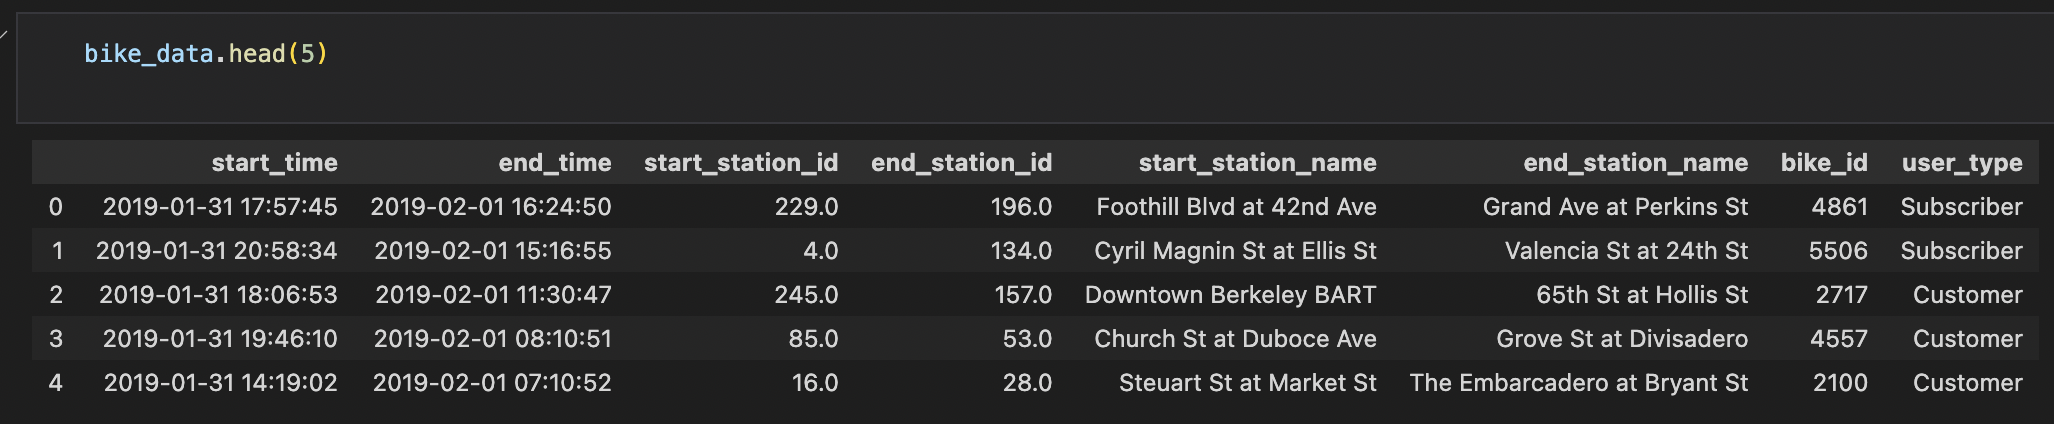
\includegraphics[width=\textwidth]{descriptive_rides.png}
    \caption{An excerpt from the trip dataset.}
    % \label{fig:png}
\end{figure}

In the first step, we examined the data for missing or incomplete values, and any duplicate entries. Thankfully, we did not find any duplicate values.

To improve our further analysis, we then added additional features to the dataset such as numeric features for \texttt{start\_hour}, \texttt{start\_weekday}, \texttt{start\_month} as well as the \texttt{trip\_duration} measured in seconds.

We then combined the external data set \href{run:../../data/Sf_2019_full.csv}{Sf\_2019\_full.csv} with the trips data set. Therefore, we created a look-up table including the \texttt{station\_id} as well as the station's actual geo coordinates from external data set and joined the geo data on the original trip data set. 
The enhanced geo features allowed us to refine the dataset to only include data from stations located in San Francisco. Trips with empty \texttt{station\_id} values are assumed to happen within the San Francisco area. That applies to around 3 \% of all trips and has a noticeable impact on the overall demand. We also removed any trips with suspicious data constellations in the trip duration as negative trip durations or outliers. We eliminated the top 0.5\% of trip durations, which were all trips that lasted longer than two hours. 

\subsection{Weather Data}
% added column names and the necessary time shift to match the trip data
The file \href{run:../../data/weather_hourly_sf.csv}{weather\_hourly\_sf.csv} gives us information about the weather in San Francisco in 2019. It includes the columns \texttt{date\_time}, \texttt{max\_temp}, \texttt{max\_temp} and the precipitation \texttt{precip}. The values of \texttt{date\_time} are UTC timestamps and needed to be shifted by -8 hours to match the ride data.

\begin{figure}[h]
    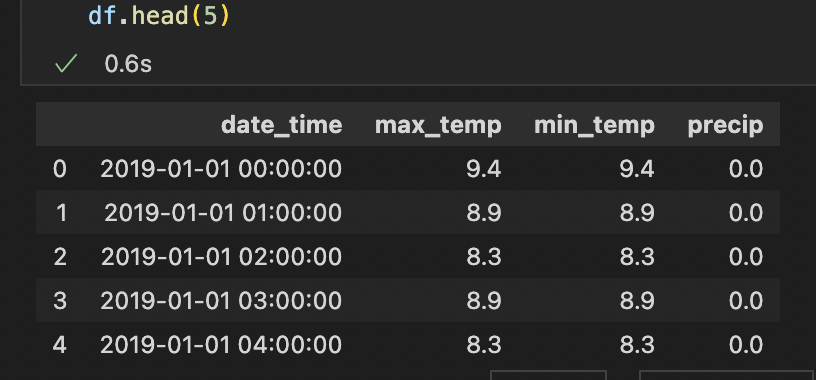
\includegraphics[width=\textwidth]{descriptive_weather.png}
    \caption{An excerpt from the weather dataset.}
    % \label{fig:png}
\end{figure}

For weather data cleaning, we checked for any missing values or duplicate entries, similar to the process used for the rides data set. We did not find any missing values, but 79 duplicate rows across all columns of the data frame and 371 duplicate entries in the \texttt{date\_time} column.

As we did not want to drop any columns easily, we determined the ratio of hourly temperature changes across the entire dataset. Temperature changes on an hourly basis at odds of roughly 2:1. The duplicated rows in the data frame can therefore be a result of duplicated entries in the \texttt{date\_time} column co-occurring with a natural steady temperature trend.
Since temperature values tend to not change within the course of an hour in non-duplicates as well, we did not declare the duplicates as redundant data. Instead, we kept the entries but adjusted the \texttt{date\_time} column by shifting these timestamps forward until no \texttt{date\_time} duplicates remain. Dropping duplicates and interpolating new values was not necessary.